\chapter{\textsc{Networks of Topics}}
\label{chapter:networks_of_topics}

The idea behind a network of topics involves two ways that the network can be constructed. Likewise, the topics within a network can be analysed from the perspective of grants as well as researchers. Technically speaking, nodes in the network will represent topics regardless of perspective. However, edges can represent either grants or researchers. In the end, two different networks of topics are constructed, the \textit{Topic-grant} network and the \textit{Topic-researcher} network.

\section{Topic-grant network}

The \textit{Topic-grant} network consists of nodes representing topics and edges representing grants. The \textit{EPSRC Research Topic Classifications} field in each grant record consists of one or more topics that classify the grant. Only grant records with two or more topics were included in the analysis. Subsequently, a link between each topic and all other topics within each grant record was established. The link signifies the grant record that the topics all have in common, and is represented as an edge in a network. Fig. \ref{figure:topic_a_structure} provides a visual explanation of how the \textit{Topic-grant} network was constructed using the collected EPSRC data, including the formulated node and edge attributes.

\begin{figure}[!htbp]
    \centering
    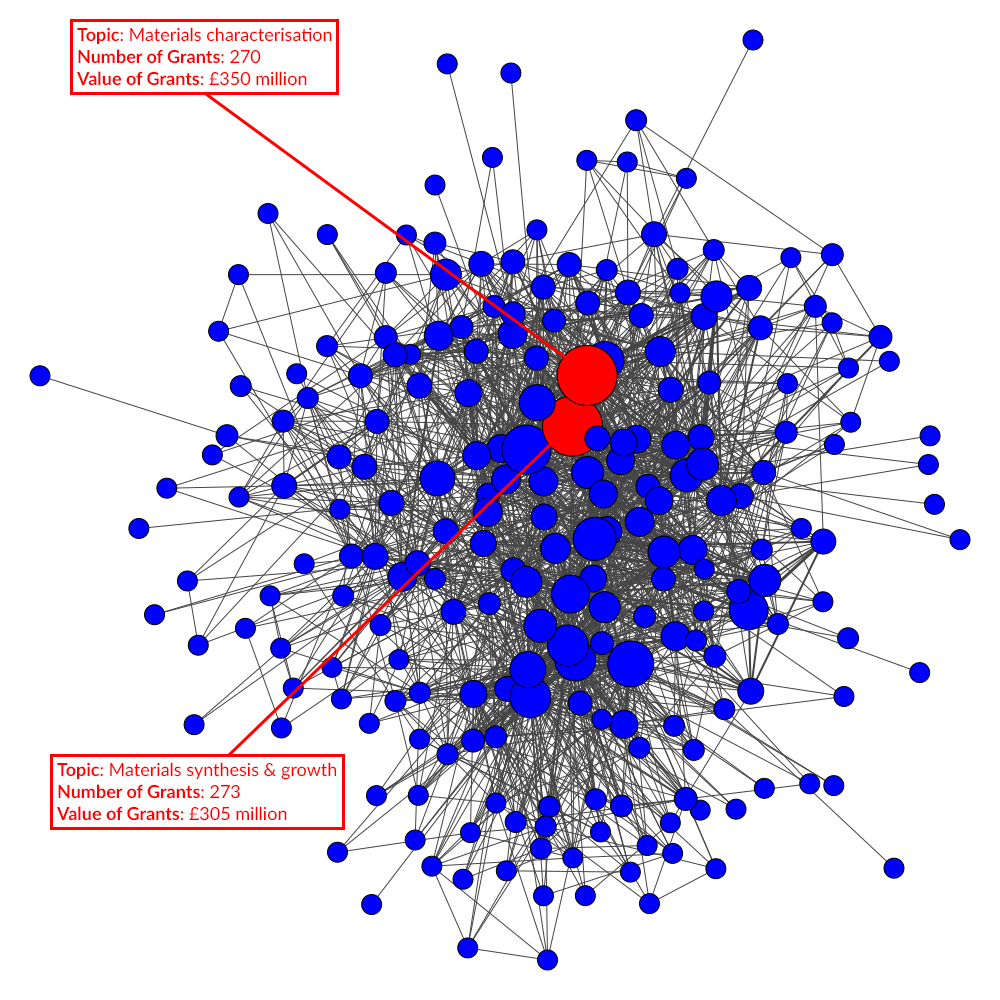
\includegraphics[width=10cm]{networks-explained/topic_network_a}
    \caption[Visual explanation of how the \textit{Topic-grant} network was structured and constructed using the collected EPSRC data]{Visual explanation of how the \textit{Topic-grant} network was structured and constructed using the collected EPSRC data, including the formulated node and edge attributes.}
    \label{figure:topic_a_structure}
\end{figure}

\subsection{Node and edge attributes}

The \textit{Topic-grant} network contains two different node and edge attributes, the number and value of grants. Node and edge attributes are common between networks. Consequently, their formulation is considered a common task, and therefore it is described in Chapter \ref{chapter:methodology}: Methodology.

\subsection{Properties of the Topic-grant network}

The \textit{Topic-grant} network constructed using the current (2010-2016) data set consists of 223 nodes representing as many topics and 2,008 edges representing common grants between topics. Table \ref{table:topic_a_properties} presents the properties of both the historical and current \textit{Topic-grant} networks.

\begin{table}[!htbp]
\centering
\caption[Properties of the \textit{Topic-grant} network constructed using both the historical (1990 to 2000, 2000 to 2010) and current (2010 to 2016) data sets]{Properties of the \textit{Topic-grant} network constructed using both the historical (1990 to 2010, 2000 to 2010) and current (2010 to 2016) data sets.}
\label{table:topic_a_properties}
\begin{tabular}{r|rrr}
{} & \textbf{1990-2000} & \textbf{2000-2010} & \textbf{2010-2016}\\
\hline\\
\textbf{Nodes}                          & {136}     & {208}     & {223}\\
\textbf{Edges}                          & {748}     & {3592}    & {2008}\\
\textbf{Type}                           & {Undirected} & {Undirected} & {Undirected}\\
\textbf{Weighted}                       & {Yes}     & {Yes}     & {Yes}\\
%\textbf{Connected}                     & {Yes}     & {No}      & {Yes}\\
\textbf{Average Degree}                 & {11}      & {34.538}  & {18.009}\\
\textbf{Average Weighted Degree}        & {12.721}  & {35.337}  & {19.543}\\
\textbf{Diameter}                       & {6}       & {5}       & {5}\\
%\textbf{Radius}                        & {3}       & {1}       & {3}\\
\textbf{Density}                        & {0.081}   & {0.167}   & {0.081}\\
\textbf{Modularity}                     & {0.4}     & {0.271}   & {0.373}\\
%\textbf{Communities}                   & {5}       & {5}       & {6}\\
%\textbf{Weak Components}                & {1}       & {2}       & {1}\\
%\textbf{Node Closeness}                & {0.392}   & {0.245}   & {0.423}\\
%\textbf{Node Betweenness}              & {108.536} & {109.776} & {156.483}\\
%\textbf{Edge Betweenness}              & {32.007}  & {12.235}  & {29.706}\\
\textbf{Average Clustering Coefficient} & {0.453}   & {0.59}    & {0.597}\\
%\textbf{Eigenvector Centrality}        & {0.105}   & {0.232}   & {0.204}\\
\textbf{Average Path Length}            & {2.54}    & {2.077}   & {2.395}\\
\end{tabular}
\end{table}

In comparison, both historical networks contain less nodes, with the \textit{2000 to 2010} and \textit{1990 to 2010} networks consisting of 208 and 136 nodes, respectively. This is expected, as the number of research topics in the past was lower, and gradually increased over time. Interestingly, the \textit{2000 to 2010} network consists of more edges which means more topics are connected through common grants. However, the increased number of edges also seems to correlate with the fact that the network is unconnected, while the other networks are connected. A network is unconnected when an edge does not exist between every pair of nodes. Furthermore, all three networks are weighted and in the creation of Table \ref{table:topic_a_properties} and Fig. \ref{figure:topic_a_current_vis}, the number of grants edge weight attribute is used.

\subsection{Visualisation of Topic-grant network}

A visualisation of the \textit{Topic-grant} network, presented in Fig. \ref{figure:topic_a_current_vis}, was produced using iGraph. It features nodes in blue, and edges in grey. The size of the node circle represents the number of grants node attribute. The width of the edge line represents the number of grants edge attribute. The topic(s) that appear in the highest number of grant records are coloured in red.

\begin{figure}[htpb]
    \centering
    \fbox{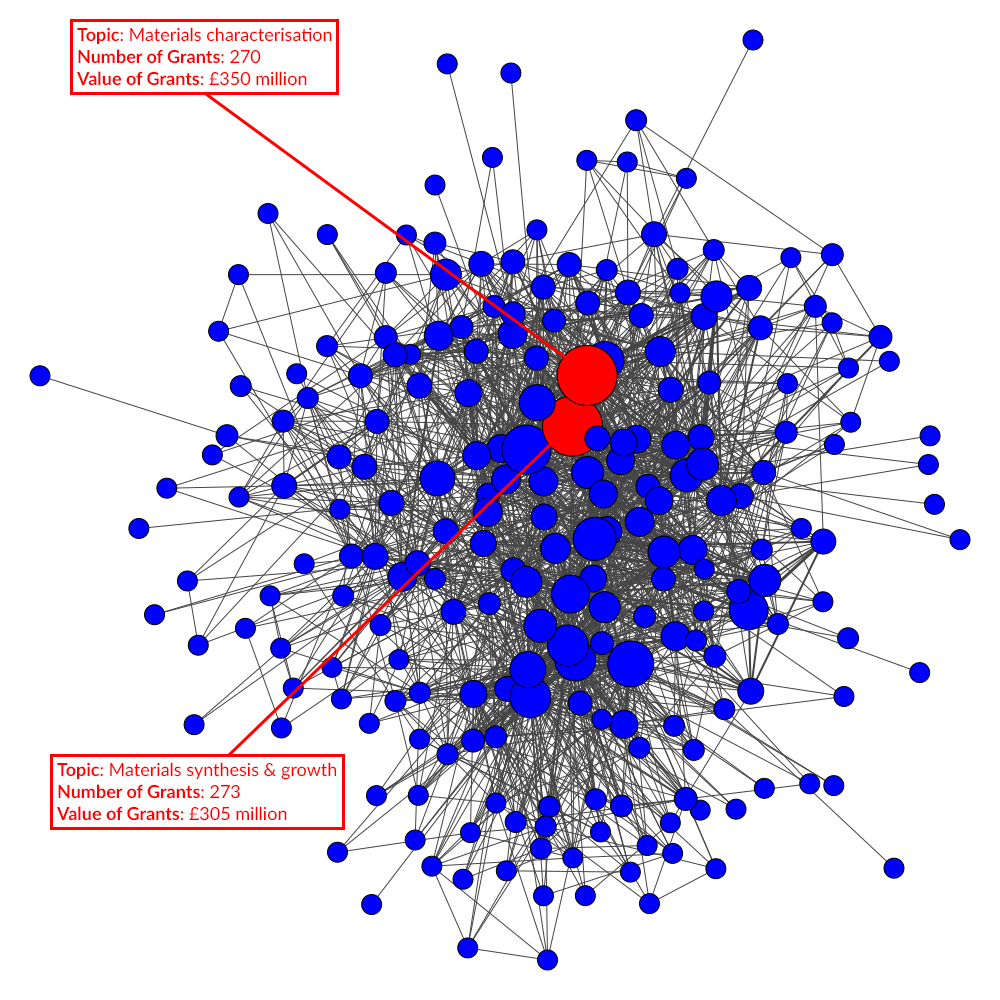
\includegraphics[width=13cm]{networks/topic_a}}
    \caption[Visualisation of \textit{Topic-grant} network constructed using the current (2010 to 2016) data set]{Visualisation of \textit{Topic-grant} network constructed using the current (2010 to 2016) data set. The topic(s) that appear in the highest number of grant records are coloured in red.}
    \label{figure:topic_a_current_vis}
\end{figure}

\section{Topic-researcher network}

The \textit{Topic-researcher} network consists of nodes representing topics and edges representing researchers. The \textit{Current EPSRC-Supported Research Topics} field in each researcher record consists of one or more topics that classify the grants supported by EPSRC that the researcher is currently an investigator in. Only researcher records with two or more topics were included in the analysis. Subsequently, a link between each topic and all other topics within each researcher record was established. The link signifies the researcher record that the topics all have in common, and is represented as an edge in a network. Fig. \ref{figure:topic_b_structure} provides a visual explanation of how the \textit{Topic-researcher} network was constructed using the collected EPSRC data, including the formulated node and edge attributes.

\begin{figure}[!htbp]
    \centering
    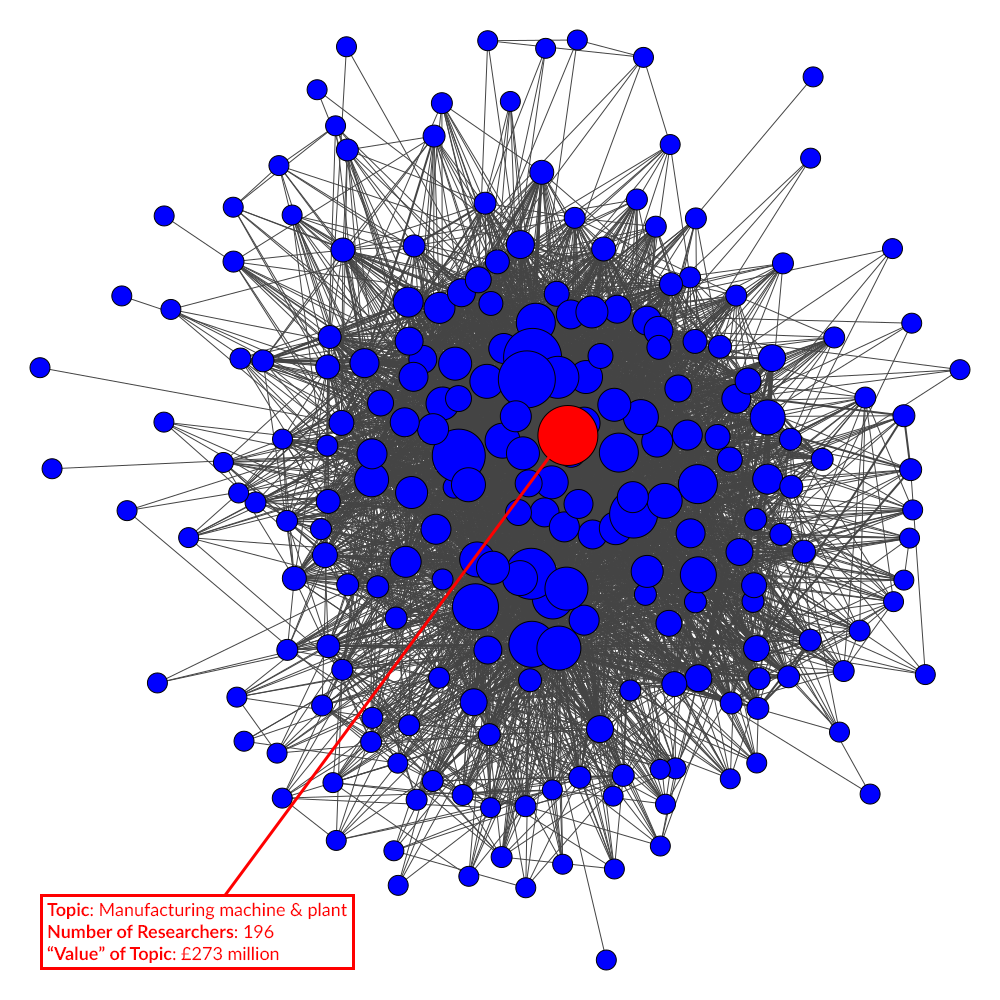
\includegraphics[width=10cm]{networks-explained/topic_network_b}
    \caption[Visual explanation of how the \textit{Topic-researcher} network was structured and constructed using the collected EPSRC data]{Visual explanation of how the \textit{Topic-researcher} network was structured and constructed using the collected EPSRC data, including the formulated node and edge attributes.}
    \label{figure:topic_b_structure}
\end{figure}

\subsection{Node and edge attributes}

The \textit{Topic-researcher} network contains one node and edge attribute, the number of grants. In the \textit{Topic-researcher network} edges represent researchers, therefore, it does not contain the value of grants attribute. Node and edge attributes are common between networks. Consequently, their formulation is considered a common task, and therefore it is described in Chapter \ref{chapter:methodology}: Methodology.

\subsection{Properties of Topic-researcher network}

The \textit{Topic-researcher} network represents the second interpretation of the topic data, and consists of topics represented by 225 nodes connected by 5,192 edges. Table \ref{table:topic_b_properties} presents the properties of the \textit{Topic-researcher} network.

\begin{table}[!htbp]
\centering
\caption[Properties of the \textit{Topic-researcher} network constructed using the current (2010 to 2016) data set]{Properties of the \textit{Topic-researcher} network constructed using the current (2010 to 2016) data set.}
\label{table:topic_b_properties}
\begin{tabular}{r|r}
{} & \textbf{2010-2016}\\
\hline\\
\textbf{Nodes}                          & {225}\\
\textbf{Edges}                          & {5192}\\
\textbf{Type}                           & {Undirected}\\
\textbf{Weighted}                       & {Yes}\\
%\textbf{Connected}                     & {Yes}\\
\textbf{Average Degree}                 & {46.151}\\
\textbf{Average Weighted Degree}        & {52.436}\\
\textbf{Diameter}                       & {4.0}\\
%\textbf{Radius}                        & {2}\\
\textbf{Density}                        & {0.206}\\
\textbf{Modularity}                     & {0.234}\\
%\textbf{Communities}                   & {4}\\
%\textbf{Weak Components}                & {1}\\
%\textbf{Node Closeness}                & {0.522}\\
%\textbf{Node Betweenness}              & {106.686}\\
%\textbf{Edge Betweenness}              & {9.477}\\
\textbf{Average Clustering Coefficient} & {0.715}\\
%\textbf{Eigenvector Centrality}        & {0.289}\\
\textbf{Average Path Length}            & {1.925}\\
\end{tabular}
\end{table}

There is a substantial increase in the number of edges compared to the \textit{Topic-grant} network. This increase is partly due to the fact that the number of researcher records (5,874) considered in the analysis exceeds the number of grant records (3,175) considered by 2,699 records. Furthermore, this network is also weighted, but this time, the edge weight represents the number of researchers two topics have in common. Moreover, the \textit{Topic-researcher network} was only constructed using the current (2010-2016) data set because researcher records only consist of the current topics of a researcher. This limits the comparison of the \textit{Topic-researcher} and \textit{Topic-grant} networks, as they can only be contrasted based on the current (2010-2016) data set.

Furthermore, it is essential to indicate the slight difference in the number of nodes between the \textit{Topic-grant} network (223 nodes) and \textit{Topic-researcher} network (225 nodes). The former considers grants with two or more topics while the latter considers researchers with two or more topics. In either network, records may exist where a specific topic appears in a single record and is also the single topic within that record. This means that the topic will not be considered in the analysis, as links to other topics cannot be established.

\subsection{Visualisation of Topic-researcher network}

A visualisation of the \textit{Topic-researcher} network, presented in Fig. \ref{figure:topic_b_current_vis}, was produced using iGraph. It features nodes in blue, and edges in grey. The size of the node circle represents the number of researchers node attribute. The width of the edge line represents the number of researchers edge attribute. The topic(s) that appear in the highest number of researcher records are coloured in red.

\begin{figure}[htpb]
    \centering
    \fbox{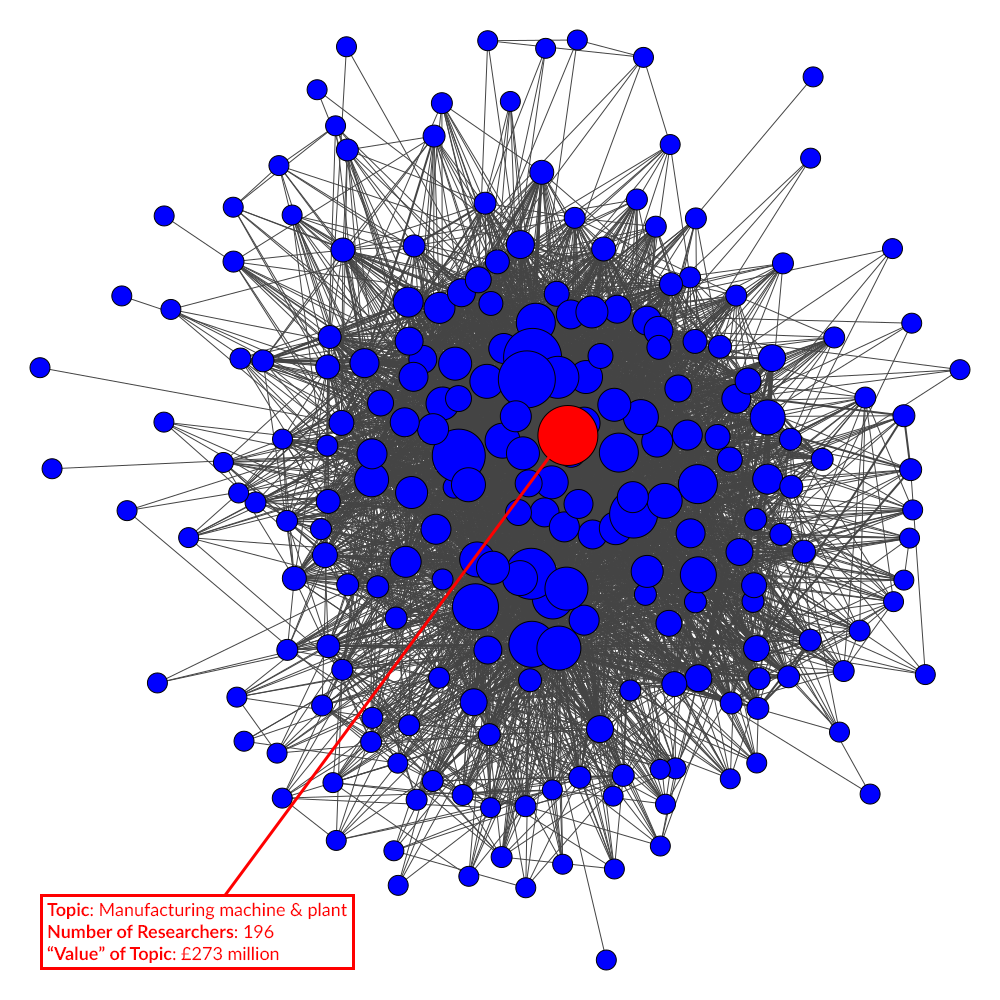
\includegraphics[width=13cm]{networks/topic_b}}
    \caption[Visualisation of \textit{Topic-researcher} network constructed using the current (2010 to 2016) data set]{Visualisation of \textit{Topic-researcher} network constructed using the current (2010 to 2016) data set. The topic(s) that appear in the highest number of researcher records are coloured in red.}
    \label{figure:topic_b_current_vis}
\end{figure}